\section{Fall 2: Auto}
\label{sec:testcase-car}
Im zweiten Testfall wird die Rekonstruktion eines Autos getestet. 
Insgesamt wurden 17 Bilder von einem schwarzen Skoda Fabia gemacht, die das Auto in verschiedenen Positionen zeigt.
Die ~\cref{tab:car-results} zeigt Anzahl der rekonstruierten Punkte pro Bildpaar.
Im Vergleich zum ersten Testfall gibt es hier deutlich weniger Matches, rekonstruierte Punkte und Punkte,die für die Skalierung verwendet worden sind.
\cref{fig:car-second-pair,fig:car-second-pair-with-matches} zeigen das zweite Bildpaar vom Auto.
Hier ist sehen, dass dass die Keypoints der meisten Matches nicht auf auf dem Auto liegen.
Stattdessen werden Matches eher an den Wänden, Pflanzen und auf dem Boden gefunden.
Bei dem Auto selbst werden die Matches hauptsächlich nur am Nummernschild und vereinzelt in den Reflexionen der Umgebung gefunden.
Wie durch die schlechten Matches zu erwarten ist, kann das Auto in den rekonstruierten Modell nicht erkannt werden, wie in \cref{fig:car-model} zu sehen ist.
In \cref{fig:car-model-2} ist das Modell aus einem anderem Winkel zu sehen.
Hier ist deutlich zu erkennen, dass die grünen Punkte der Pflanzen im Hintergrund in der gleichen Ebene wie viele andere Punkte liegen. 
Dies lässt auf einen Fehler in der Triangulation oder Skalierung der Punkte vermuten.

\begin{table}
    \begin{tabularx}{\textwidth}{cXXXX}
        \toprule
        Bildpaar &  Anzahl der Matches & Anzahl der Weltpunkte & Anzahl der Weltpunkte für Skalierung & angewandte Skalierung \\ 
        \midrule
        \makecell[r]{1} & \makecell[r]{575} & \makecell[r]{480} & \makecell[r]{-}  & \makecell[r]{-} \\
        \makecell[r]{2} & \makecell[r]{910} & \makecell[r]{860} & \makecell[r]{165} & \makecell[r]{0,468641} \\
        \makecell[r]{3} & \makecell[r]{685} & \makecell[r]{653} & \makecell[r]{227} & \makecell[r]{0,768563} \\
        \makecell[r]{4} & \makecell[r]{583} & \makecell[r]{570} & \makecell[r]{51}  & \makecell[r]{0,788242} \\
        \makecell[r]{5} & \makecell[r]{264} & \makecell[r]{247} & \makecell[r]{25}  & \makecell[r]{0,60277} \\
        \makecell[r]{6} & \makecell[r]{427} & \makecell[r]{409} & \makecell[r]{58}  & \makecell[r]{0,848896} \\
        \makecell[r]{7} & \makecell[r]{393} & \makecell[r]{346} & \makecell[r]{95}  & \makecell[r]{2,80038} \\
        \makecell[r]{8} & \makecell[r]{799} & \makecell[r]{527} & \makecell[r]{99}  & \makecell[r]{0,923119} \\
        \makecell[r]{9} & \makecell[r]{827} & \makecell[r]{518} & \makecell[r]{113} & \makecell[r]{0,577807} \\
        \makecell[r]{10} & \makecell[r]{618} & \makecell[r]{597} & \makecell[r]{125} & \makecell[r]{1,11263} \\
        \makecell[r]{11} & \makecell[r]{251} & \makecell[r]{187} & \makecell[r]{56}  & \makecell[r]{0,472208} \\
        \makecell[r]{12} & \makecell[r]{68}  & \makecell[r]{36}  & \makecell[r]{10}  & \makecell[r]{1,49154} \\
        \makecell[r]{13} & \makecell[r]{341} & \makecell[r]{325} & \makecell[r]{2}   & \makecell[r]{1,33112} \\
        \makecell[r]{14} & \makecell[r]{334} & \makecell[r]{263} & \makecell[r]{18}  & \makecell[r]{2,02715} \\
        \makecell[r]{15} & \makecell[r]{175} & \makecell[r]{166} & \makecell[r]{12}  & \makecell[r]{0,475839} \\
        \makecell[r]{16} & \makecell[r]{167} & \makecell[r]{146} & \makecell[r]{21}  & \makecell[r]{0,651284} \\
        \midrule
        Summe & \makecell[r]{7.417} & \makecell[r]{6.330} & \makecell[r]{1.077} & \makecell[r]{-} \\
        \bottomrule
    \end{tabularx}
    \caption{Ergebnis der Rekonstruktion der Autobilder.}
    \label{tab:car-results}
\end{table}

\begin{figure}[b]
    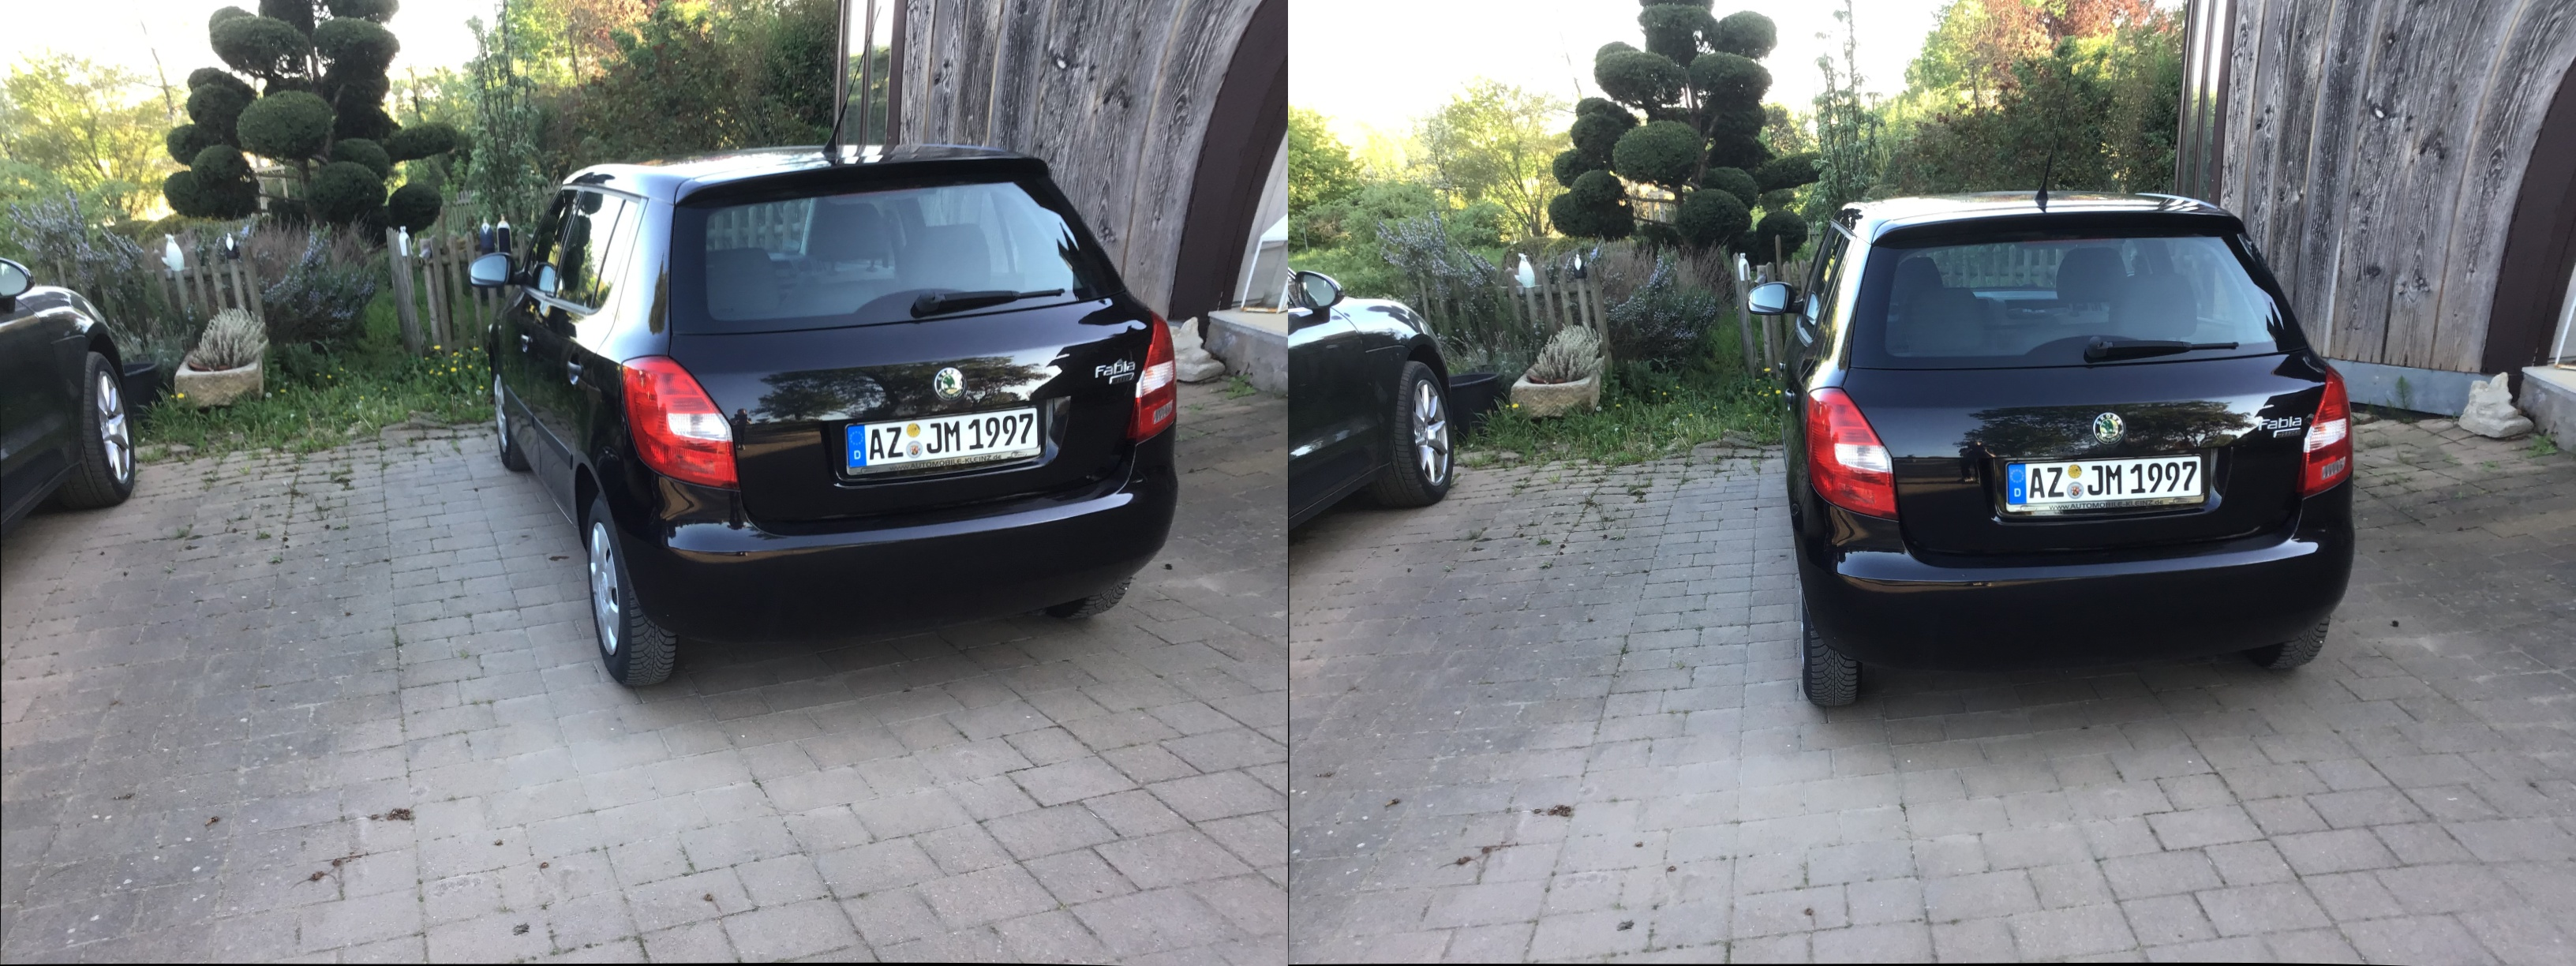
\includegraphics[width=\textwidth]{src/img/car_second_pair.jpg}
    \caption{Das zweite Bildpaar zum Rekonstruieren des Autos.}
    \label{fig:car-second-pair}
\end{figure}

\begin{figure}
    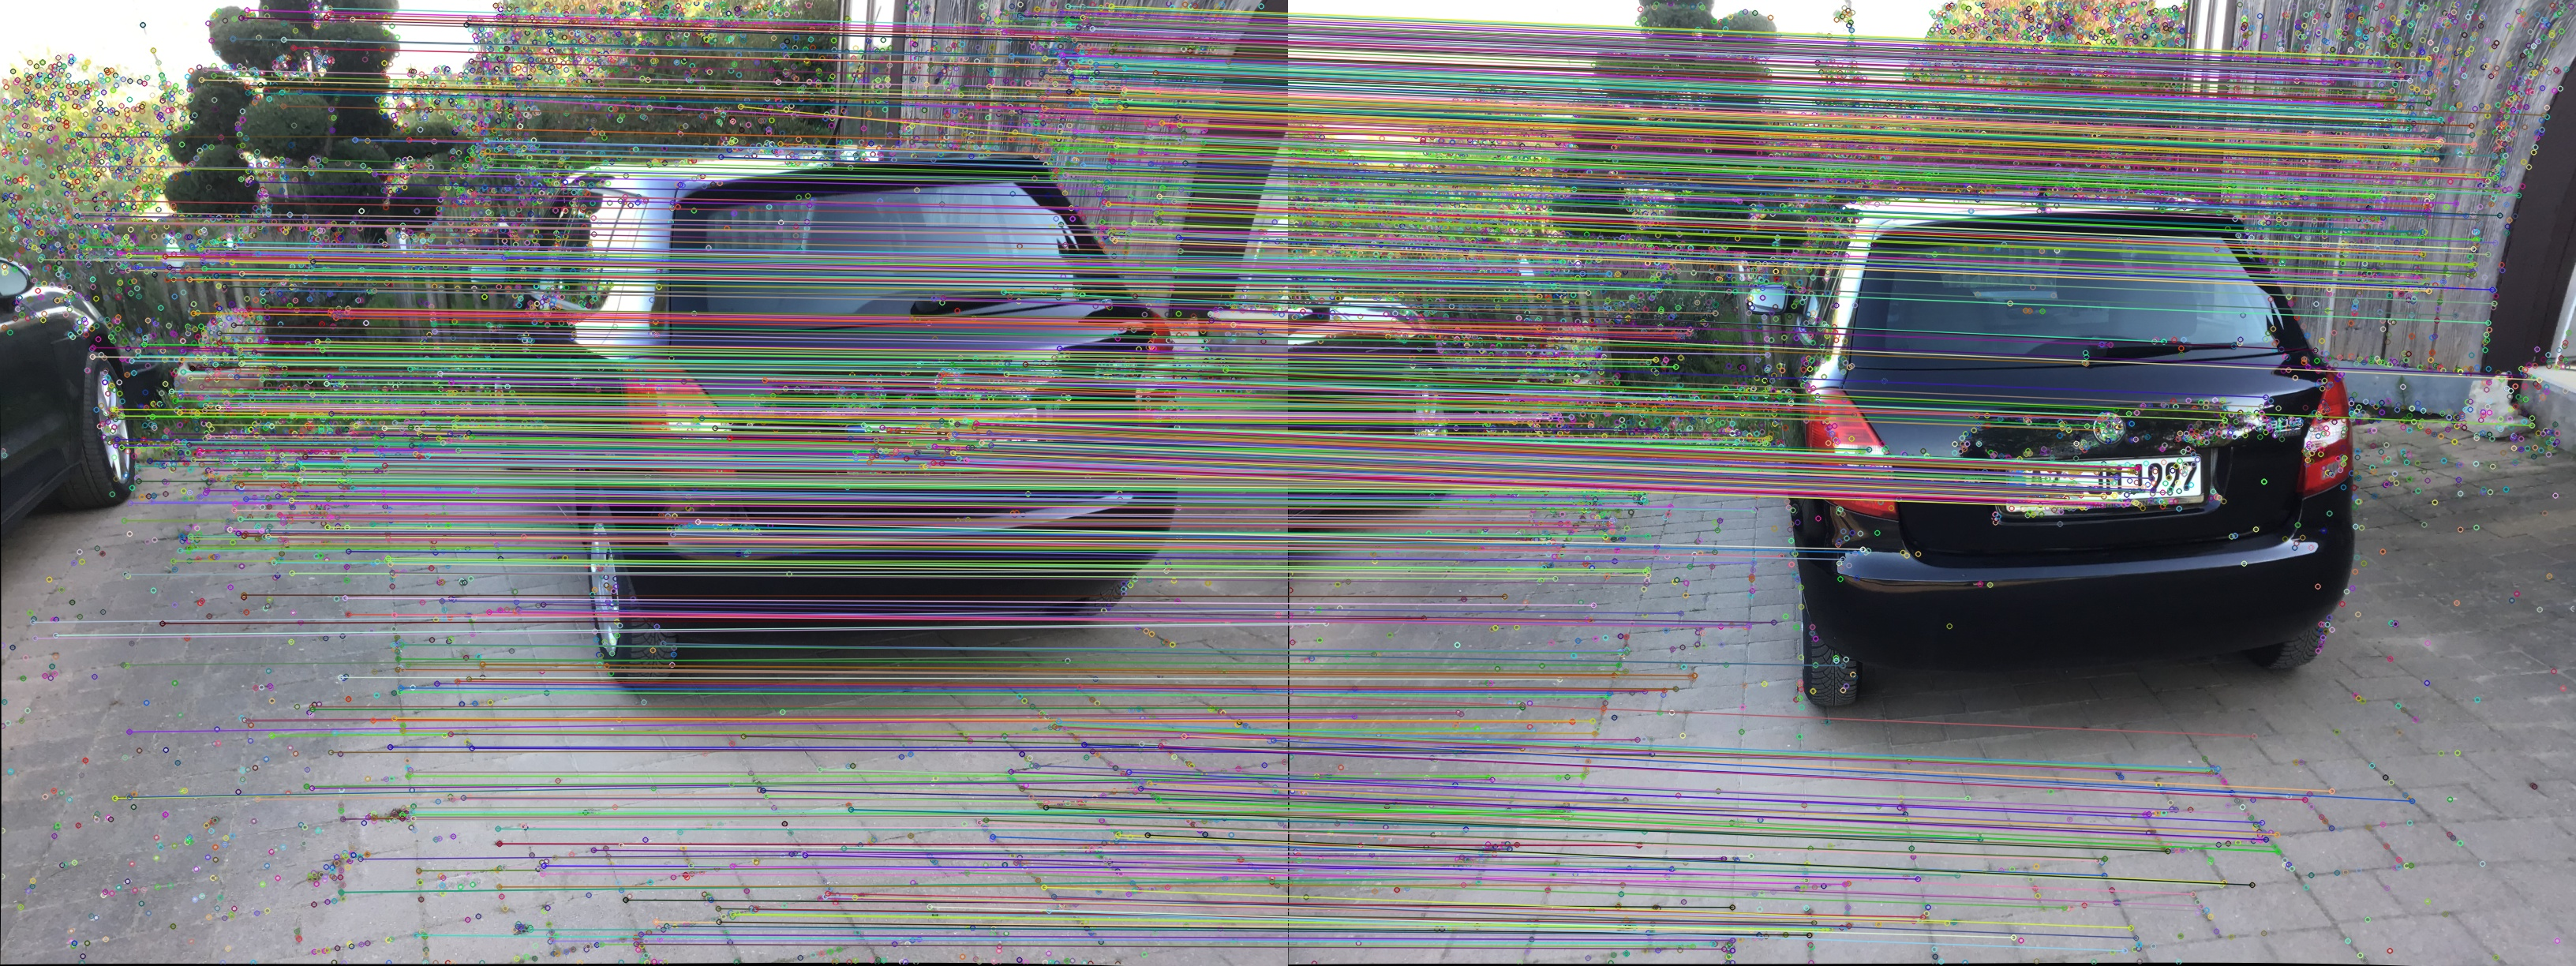
\includegraphics[width=\textwidth]{src/img/car_second_pair_with_matches.jpg}
    \caption{Das zweite Bildpaar vom Auto mit Keypoints und Matches.}
    \label{fig:car-second-pair-with-matches}
\end{figure}

\begin{figure}
    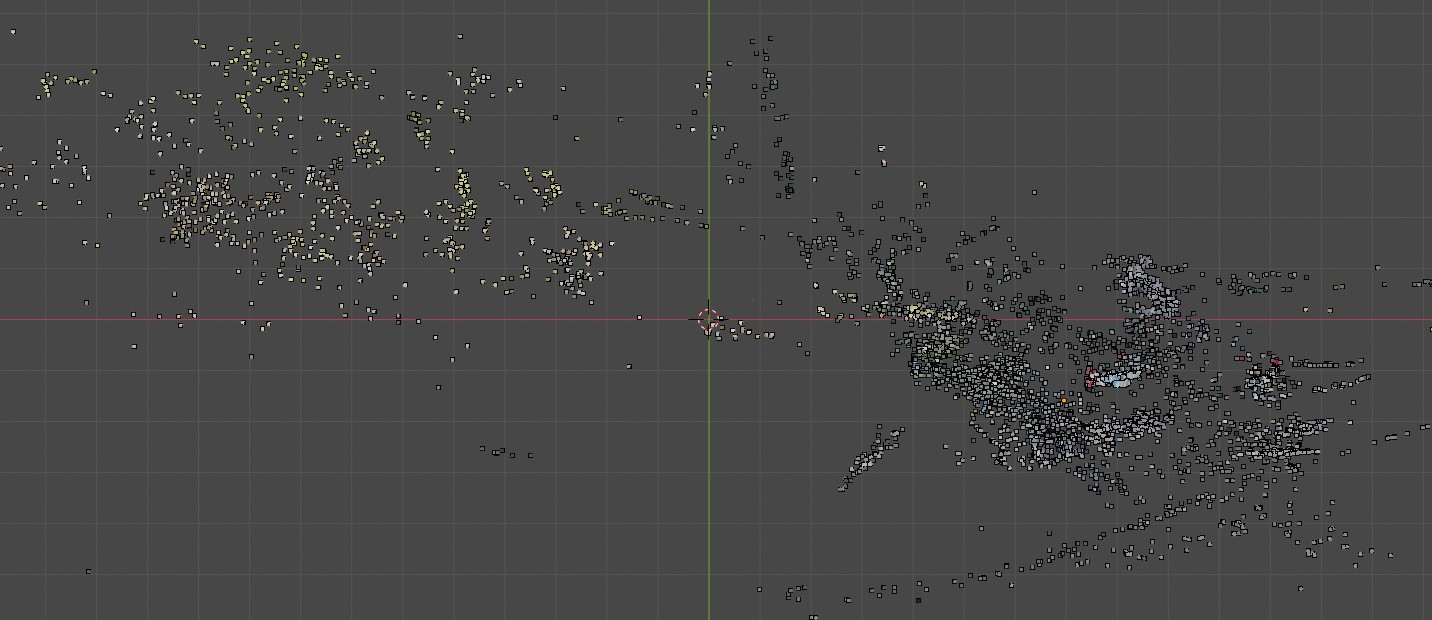
\includegraphics[width=\textwidth]{src/img/car_model.jpg}
    \caption{Die rekonstruierten Matches des Autos. Das Bild zeigt das Model aus der Sicht der ersten Kamera.}
    \label{fig:car-model}
\end{figure}

\begin{figure}
    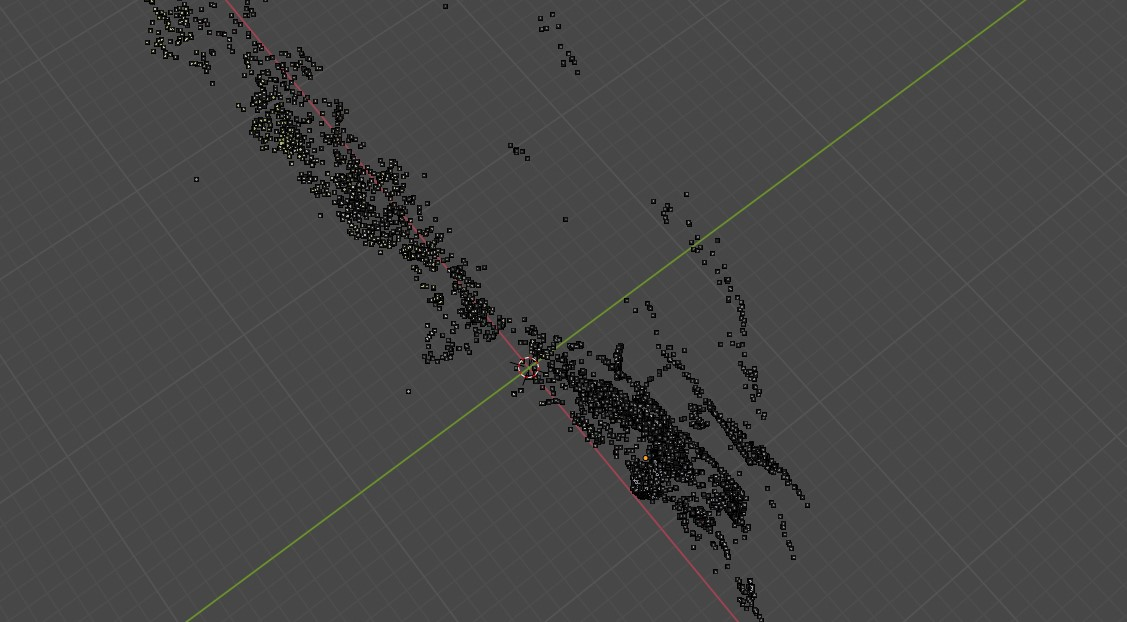
\includegraphics[width=\textwidth]{src/img/car_model_2.jpg}
    \caption{Die rekonstruierten Matches des Autos. Das Bild zeigt das Model von der Seite.}
    \label{fig:car-model-2}
\end{figure}
